One of the mains features of this work is to have demonstrated that, independently of its condition, microbiota follows Taylor's law. We have seen that the value of the scaling index in each case is always less than the unity (using standard deviation as the measurement for dispersion), which provides us with information about the community structure. This means that, in relative terms, the most abundant elements in the population are less volatile to perturbations than the less abundant ones. The explanation for this universal pattern is not clear although some hypotheses have been tested in other studies, such as the presence of negative interactions in the population \cite{kilpatrick}, and a demonstration that this may depend on reproductive correlation \cite{ballantyne}. Nevertheless, none of these explanations are sufficient when we are talking about microbiota, as the reproduction term is diffuse, the interactions between its components are not only based on competition \cite{joao, mehta, bucci}, and that even that kind of negative interaction may not effectively yield values less than the unity when referring to a bacterial species \cite{ramslayer}. Anyhow, the values obtained in all cases were very similar from one to another, which could suggest that the community structure is preserved throughout the different scenarios we studied.

The second parameter provides information about noise and can be directly linked to the variability or fluctuation amplitude of the population over time. It is a direct estimator of the stability of the system under study. As we have shown above, the healthy subset of each study has lower variability than the non--healthy subset, when dealing with adult individuals. Interestingly, the variability parameter was higher in the healthy subset in the study of the discordant twins suffering from kwashiorkor disease \cite{kwashiorkor}. In this regard, it has been shown that infant microbiota needs to develop toward a definite, adult state \cite{koenig}. This implies that temporal variability is greater in children compared to a healthy adult state, which should be temporally stable. Thus, our results could point to the need for this variability in order to reach that adult state. Furthermore, as we wanted to see how this variability behaved over time, we calculated the evolution of this parameter for the samples which had enough time sampling. As shown in Figure \ref{fig:tempevo1}, the variability of microbiota fluctuated over time. It is interesting to note in Figure \ref{fig:tempevo2} how this parameter captured the two antibiotic intakes in one of the patients from the study by Dethlefsen and Relman \cite{antibiotic}, especially in that there seems to be some kind of a resilience process in the microbiota due to the lower variability increase in the second antibiotic intake.  

The primary hypothesis of this work is that, in adults, having a healthy microbiota means that the population is stable over time and does not move into a state where it is highly susceptible to external or internal perturbations, causing a dysbiotic state in the microbiota. In order to use the valuable information provided by the empirical law of Taylor's work, we proposed the use of Langevin's equation to model how ranking stability evolved over time. While the system noise component can be directly measured as its variability, the other main term needs to be inferred from the model. This term, which we named "fitness", is the one that enables the system to be stable in the face of potential perturbations. In ecological terms, this could represent the nature of interactions that are present among bacteria, between bacteria and other minority populations, such as fungi or archaea, between bacteria and the viral component in microbiota, and interactions between the host and the whole microbiota. As this is a first step to model the temporal stability of microbiota, and given its complex nature, we calculated fitness using the Fluctuation Dissipation Theorem as a first approximation\cite{FD}. Thus, the fitness of microbiota will still need to be modeled in future works in order to make the model more accurate and give it a higher predictive power. 

By solving Langevin's differential equation, we can obtain a phase diagram where each microbiota sample can be placed according to its fitness and variability into one of two phases, according to the ranking stability of the system. As we can see in the phase--space in Figure \ref{fig:main3}, three different conditions that could occur are shown. First, we could have a healthy microbiota with some fluctuations, as shown by one of the subjects of Caporaso \emph{et al.}'s study \cite{moving}. Because this case would have good fitness, its temporal variability would not place the microbiota in the unstable phase of the diagram. Second, we have a subject from the study by Dethlefsen and Relman \cite{antibiotic} who was perturbed twice by an antibiotic intake. His microbiota underwent sufficient change so as to lose its stability, and hence be placed in the unstable part. In this location, it is more sensitive to potential perturbations such as, for example, opportunist infections. In the third and last condition, the subject was already in the unstable phase due to a health issue, i.e. IBS. This can be observed in one of the patients from Durban \emph{et al.}'s study \cite{IBS}. In addition, it was shown that this subject's health status improved during the time the experiment was carried out, implying that his microbiota also recovered the stability it had lost. It is interesting to note that in the subject's health from the study made by David \emph{et al.} \cite{hostlife} who suffered a Salmonella infection during the experiment, there was a significant shift in variability and a final recovery from the perturbed state (see Supplementary Figure S\ref{supfig:HLS_xWSummary}).

\begin{supfig}
	\centering
	%\vspace*{-10mm} % Corrects overbox of the figures
	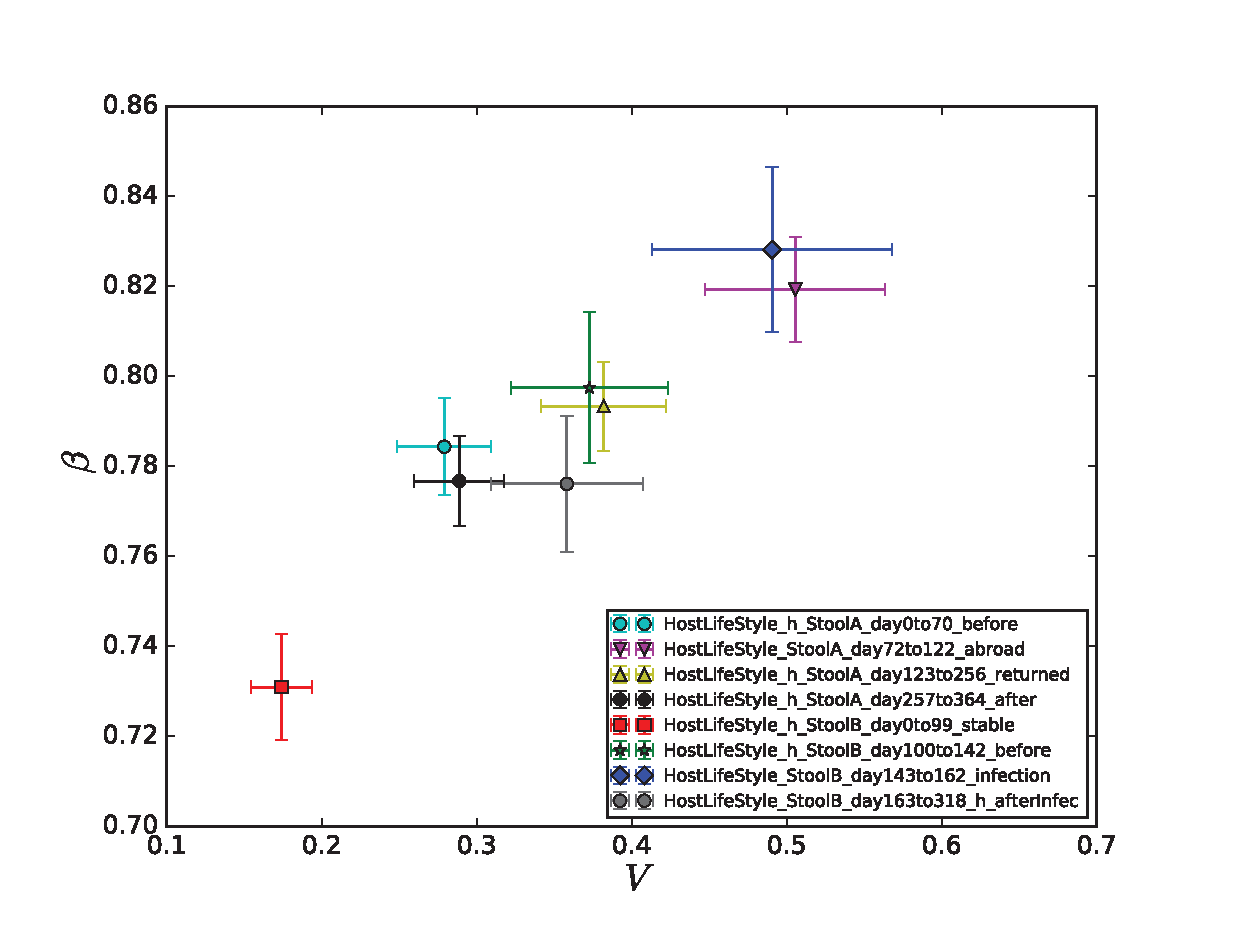
\includegraphics[width=0.99\textwidth]{figs/supfig_HLS_xWSummary.eps}
	\caption{Taylor's law parameter space for intervals concerning gut microbiota in the host lifestyle study\cite{hostlife}. We observe that subject \emph{B}, who suffered a Salmonella infection during the experiment, had a relevant shift in the parameters from \emph{\_before} to \emph{\_infection} and a final recovery from the perturbed state to \emph{\_afterinfec}, which lies in the parameter area compatible with the healthy and stable intervals (see Supplementary Table S\ref{tab:Ab-IBS-HLS}). Subject \emph{A} also had a shift in variability from \emph{\_before} to \emph{\_abroad} and back to \emph{\_returned}, also in the proximity zone of healthy and stable periods.}
	\label{supfig:HLS_xWSummary}
\end{supfig}
 
Specifically, the analysis of the rank stability of different periods of time belonging to the individual \emph{A} in the host lifestyle study \cite{hostlife}, suggests that the presence of \emph{rank stability islands} among medium-ranked taxa is an interesting feature. Interestingly, this stability was compromised when the period was not an ordinary one, suggesting that those taxa were sensitive to changes in the lifestyle. Among the genera identified as \emph{rank stability islands}, \emph{Lachnobacterium} and \emph{Clostridium} were catalogued as genera predictive of dysbiosis in the work of Larsen and Dai \cite{rsi_dysbiosis}, which analysed the same dataset \cite{hostlife}. Furthermore, very recently, it has been confirmed a clear relationship between \emph{Actinomyces} and conventional adenoma \cite{rsi_actino}, one of the two main precursors of the colorectal cancer. Finally, \emph{Eggerthella} is an opportunistic pathogen that is often associated with serious gastrointestinal pathology \cite{rsi_egg}.

It could be brought into question the role of these taxa as key players in the phase transition of the microbiota, or whether they are more susceptible to perturbations than the most abundant. The types of interactions that could sustain this particular behavior are not clear, as these non-abundant taxa are not usually included in dynamic studies in order to obtain a community matrix. Further experiments and data analysis are needed to clarify whether \emph{rank stability islands} are a widespread feature of microbiotas and whether they appear at lower taxonomic levels too.

However, we have to be aware that the hypothesis above is too simplistic to be directly related to reality. It has been demonstrated that the situation is more complex than the outlook provided which separate healthy people from non-healthy people just by compositional terms, as Moya and Ferrer underlined in their recent review \cite{Moya_trends}. There are several different feasible scenarios in which we can consider microbiota as being stablem irrespective of their compositional evolution over time. For example, depending on its ability to recover its initial composition (resilience), or whether it can recover its original function despite its composition (functional redundancy). What we have shown in this work could be explained as the transition of stable microbiota into a state of dysbiosis.  

As a first step towards understanding microbiota stability, the model presents some limitations and there is still work to do. From a biological perspective, many questions arise from this work. We have observed the same pattern in Taylor's parameters in all the different conditions we studied, but a pertinent question is whether this is really a universal feature in the huge diversity of microbial niches. Furthermore, another relevant question centers on which mechanisms are involved in maintaining the population structure. The nature of the interactions between the elements of community is surely of great importance in this matter, and this is related to the fitness of the community, as mentioned above. How we should address community fitness is not clear, but works such as the one by Tikhonov \cite{tikhonov} could point us in the right direction to unravel the complexity of microbiota.